% This file contains the sections, paragraphs, and figures I deleted
% after a first-pass on 2023-08-24.

% From synthetic oscillations report
In the time series analysis literature, there is a wealth of analysis methods that aim to find parameters pertaining to the periodicity of noisy time series and that aim to characterise the relationship between two signals.
This is relevant for biological time series, especially because they are noisy due to both intrinsic and extrinsic noise sources, and because researchers often record multiple time series from the same system to study the relationship between such time series.
One example is the yeast metabolic cycle, which is known to be a metabolic oscillator that is coupled with the cell division cycle oscillator.
In this case, the two time series from this system consist of the level of metabolites to represent the metabolic oscillator and the activity of a component of the cell division cycle to represent the cell division cycle.

The first step of any data science pipeline is cleaning data.% , and of course there is the adage: 80\% of data science is cleaning data [CITATION NEEDED].
Cleaning data is important because of `garbage in, garbage out': regardless of how cutting-edge the analysis methods are, if the input data is flawed, the data analyst cannot obtain good insights from the data.
However, this step involves judgement calls: the analyst needs to decide on criteria to separate useful data from useless data.
These criteria may be based on existing standards of practice or, for systems biology, knowledge of either the underlying biological processes or of the mathematical constraints.
Often, these criteria can be arbitrary because there is an absence of existing standards of practice for the specific situation --- in this case, any decision is going to be a trade-off and needs justification.

\begin{figure}
  \centering
  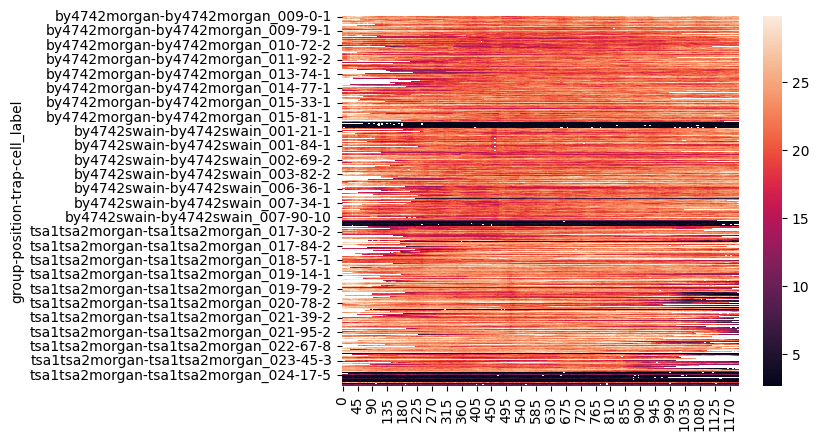
\includegraphics[width=0.9\textwidth]{example_dataframe_heatmap}
  \caption[
    Heatmap of example dataframe
  ]{
    Heatmap of example dataframe shown in figure~\ref{fig:analysis-example-dataframe}.
    Each row represents a cell, each column represents a time point, and the colour of the pixel (colour bar, right) represents the fluorescence intensity.
    Some cells are not present for the whole time course of the experiment, and errors in the segmentation pipeline produce missing time points seen as white pixels in the heatmap.
  }
  \label{fig:analysis-example-heatmap}
\end{figure}

For example, in climate science, if there is a time series of atmospheric \ce{CO2} over a period of decades, we would like to filter out the annual (seasonal) cycles and look at the long-term changes over time.

Next, missing time points can pose a problem, especially when many analysis methods assume evenly-spaced time series. %[WHICH?]
The Lomb-Scargle periodogram \parencite{lombLeastsquaresFrequencyAnalysis1976} is a method developed for problems like this.
Specifically, it was developed for astronomical data that often has missing time points, corresponding to cloud cover, for example.
In my analysis, cases of missing time points are few and could be resolved by linear interpolation, so I will not discuss in detail methods to handle missing time points.


The spectra (figure~\ref{fig:analysis-svc-fft}) suggest that oscillatory cells exhibit a peak, corresponding to features 6--7, that is absent in non-oscillatory cells.
The peak corresponds to a period of 70--80 minutes.
This peak may explain the good precision \& recall scores.

\begin{figure}
  \centering
  \begin{subfigure}[htpb]{0.7\textwidth}
   \centering
   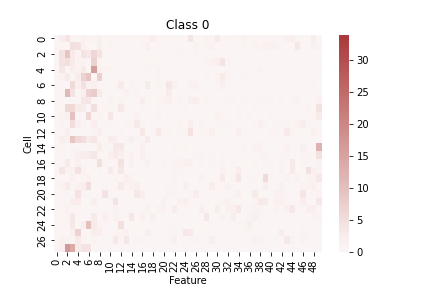
\includegraphics[width=\textwidth]{fft_testing_featurevector_0}
   \caption{
   }
   \label{fig:analysis-svc-fft-0}
  \end{subfigure}

  \begin{subfigure}[htpb]{0.7\textwidth}
   \centering
   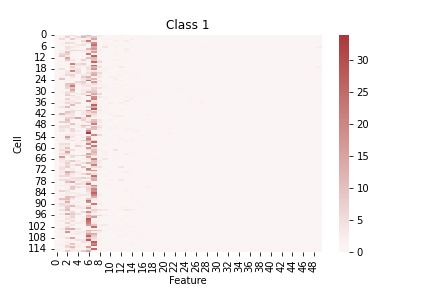
\includegraphics[width=\textwidth]{fft_testing_featurevector_1}
   \caption{
   }
   \label{fig:analysis-svc-fft-1}
  \end{subfigure}
  \caption[
    Fourier spectra of cells in testing set
  ]{
    Fourier spectra of cells in testing set classified as non-oscillatory (class 0,~\ref{fig:analysis-svc-fft-0}) and oscillatory (class 1,~\ref{fig:analysis-svc-fft-1}) by an SVC.
    Rows represent each cell, each used as an observation for the model.
    Columns represent each discrete frequency, used as a features for the model.
    Shades of red represent the power at each discrete frequency, used as feature values.
  }
  \label{fig:analysis-svc-fft}
\end{figure}


\textcite{zielinskiStrengthsLimitationsPeriod2014} discuss several methods, including: FFT NLLS (non-linear least squares, described by \textcite{straumeLeastSquaresAnalysisFluorescence2002}), MFourFit \parencite{edwardsQuantitativeAnalysisRegulatory2010}, MESA (maximum entropy spectral analysis, described by \textcite{burgRelationshipMaximumEntropy1972}), and the Lomb-Scargle periodogram \parencite{lombLeastsquaresFrequencyAnalysis1976}.

% I probably need to try out at least the first two
\begin{description}
    \item [FFT NLLS] \hfill \\

        \begin{itemize}
          \item Is based on the assumption that the time series is best modelled by a sum of cosine functions, each with its own period, amplitude, and phase.
                In general, five cosines are sufficient for most biological data.
          \item First fits the data with one cosine and adjust the period, amplitude, and noise parameters using the non-linear least squares fitting algorithm.
                The Fast Fourier Transform (FFT) can be performed to find a good set of initial parameters.
                Subsequent cosines are added and their parameters found using the same process until new cosines do not significantly improve the fit.
          \item The confidence levels of the parameters are found by varying the parameter values until the resulting fit significantly differs from the best-fit model.
                These can be expressed in terms relative to the original best-fit parameter values.
          \item The period of the time series is reported as the period of the cosine that gives the best fit and is within the expected range of periods.
                Skewness does not affect period.
        \end{itemize}

    \item [MFourFit] \hfill \\

        \begin{itemize}
          \item Is based on fitting one principal cosine and up to four additional cosines, as a way to reduce model complexity.
                Each cosine has a period, amplitude, and phase parameter, but the phase parameters of each additional cosine is define as a fraction $\frac{1}{2}, \frac{1}{3}, \ldots \frac{1}{5}$ of the principal cosine.  These harmonics describe the shape of oscillations.
          \item This algorithm does not directly estimate a period, but varies its estimating of the period within a range of user-defined values.
                The algorithm evaluates the fit by computing the sum of squared differences between the model and the data, and the model is chosen based on the best fit.
          \item This algorithm always returns a period even if the time series is not oscillatory.
                It also assumes knowledge of the shape, and skewness does not affect period.
        \end{itemize}

    \item [MESA] \hfill \\

        \begin{itemize}
          \item Unlike previous curve-fitting methods, MESA fits an autoregressive model to the data then gets period from it.
                The autoregressive model assumes that each data point can be expressed as the linear combination of a defined number of time points before it (the order), plus noise.
                This fitted model leads to an analytical expression of the frequency spectrum, and the period can be found from this expression.
          \item Choosing the best order can be a form of model selection.
          \item Does not assume a shape of the waveform, and is more precise that Fourier-based methods, but lacks a confidence measure.
                Empirically does well and fast.
                It is based on a very different principle than MFourFit, so if both methods agree on the value of the period, then we can be confident that we have the correct period.
        \end{itemize}

    \item [Lomb-Scargle periodogram] \hfill \\

        \begin{itemize}
            \item Fits one sinusoid, assumes a period.
            \item Choose one that gives least error.
            \item Can be used with data with time points that are not evenly spaced
        \end{itemize}

\end{description}

For further detail, I discussed MESA in section~\ref{subsec:analysis-classification-ar} and the Lomb-Scargle periodogram in section~\ref{subsec:analysis-classification-spectral}.

% First-order DEs redundant?
or as a system of first-order differential equations:

\begin{equation}
  \begin{aligned}
    \ndif{y}{t} &= v \\
    \ndif{v}{t} &= -\omega^{2}y
  \end{aligned}
  \label{eq:harmonic-1o}
\end{equation}


\subsubsection{Summary}
\label{subsubsec:analysis-characterisation-acf-summary}

My investigation aims to address a signal processing question.
Therefore, for the purposes of my investigation, it is not important that these oscillators function as an accurate model of the biological systems responsible for the biological oscillations observed.
Indeed, given that 47 flavoproteins are responsible for flavin autofluorescence, a component of such a poorly biochemically characterised system like the yeast metabolic cycle, it is not feasible to find a mathematical model that accurately describes the biological oscillations.

The methods developed for the biological timekeeping field, especially circadian rhythms, tend to symmetrical, sinusoidal time series.
However, many such methods do not suit skewed oscillations such as the FitzHugh-Nagumo oscillator, which models histone 2B abundance changes in the cell division cycle, therefore other methods must be used.
The autocorrelation function has previously been used to evaluate the periodicity of time series in the yeast metabolic cycle, and here I show that this function can additionally be used to quantify noise properties of the time series.
However, this function has limited ability of quantify the noise timescale of the FitzHugh-Nagumo oscillator.

Potentially, this investigation can be extended to oscillators modelled by other systems of differential equations that describe other biological rhythms.


% MORE
% --------------

The problem with applying classical time series analysis methods to biological time series lies with two properties of biological time series: they are noisy and they are often short.
Classical methods such as Fourier analysis have been shown to be useful in characterising noisy biological time series when they are long, e.g.\ from neuron impulse recordings, which can include up to thousands of oscillations.
However, for examples such as the yeast metabolic cycle, it is not feasible to record time series that include such a high number of oscillations.
In this case, 5-10 oscillations are more realistic.
As a result, methods like Fourier analysis only provide poor resolution for characteristics such as the period of oscillations.

To discuss the process of analysing oscillatory time series in more detail, I will be using my data as an example and divide this chapter according to steps in the process (see figure~\ref{fig:analysis-data-overview}).
My data consists of 100--1000 time series of recorded flavin intensity changes for each cell, indicating the yeast metabolic cycle.
Some experiments include HTB2::mCherry strain cells, and I obtain both flavin intensity changes and mCherry intensity changes from each cell;
the mCherry indicating the cell division cycle.
In these time series, there is a new time point every 5 minutes, for a total of 100--300 time points.
These data are stored as dataframes for each condition (strain and media conditions), with the time series as rows and time points as columns ---
in the case of HTB2::mCherry cells, the flavin and mCherry time series are in separate data tables.


Three problems I occur in my data are: choosing data, time series filtering, and handling missing time points.
As context to illustrate my problem, figure~\ref{fig:analysis-example-heatmap} presents raw data from an example experiment.

The first step is choosing data.
This is handled in the analysis pipeline \textit{aliby} by the \textit{picker} process, which removes time series that correspond to objects other than living cells and subsequently chooses time series that have time points present for at least 80\% of the total time points \parencite{munozgonzalezPhenotypingSingleCells2023}.
This is an arbitrary cut-off, but it ensures that my time series have enough oscillations for further analysis, such as characterisation of the frequencies of these oscillations.
Otherwise, short, and likely uninformative, time series can `pollute' algorithms that operate on the population of time series, confounding the analysis.
Some time series have missing time points.
The \textit{merger} process in \textit{aliby} resolves errors in cell tracking across time points by merging short tracks previously identified in the pipeline as belonging to separate cells.
Missing time points arise from errors even after \textit{merger} runs, but are few enough that simple linear interpolation can resolve the majority of cases.

\begin{figure}
  \centering
  \begin{subfigure}[htpb]{0.8\textwidth}
   \centering
   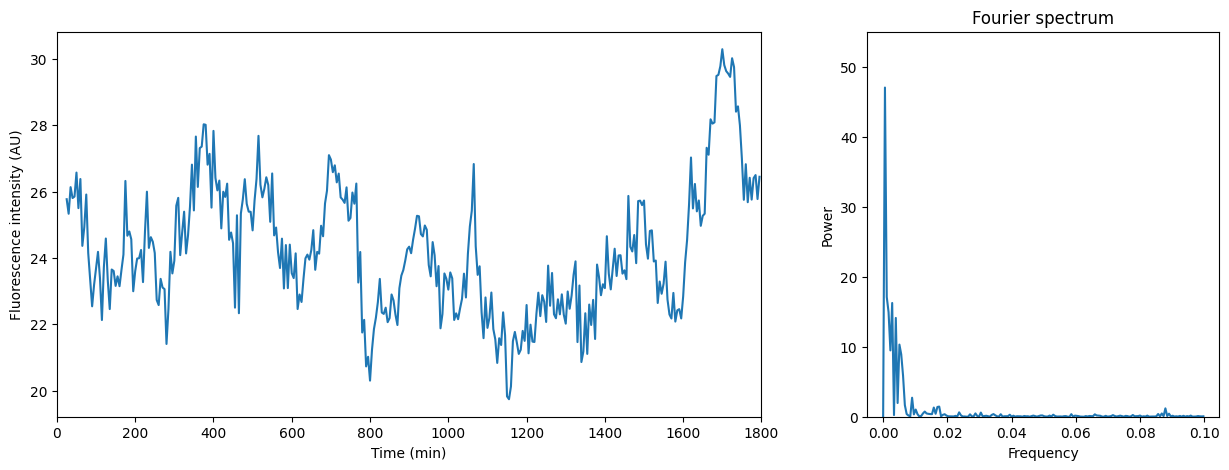
\includegraphics[width=\textwidth]{fft_raw}
   \caption{
     Raw signal
   }
   \label{fig:analysis-filter-raw}
  \end{subfigure}
  \begin{subfigure}[htpb]{0.8\textwidth}
   \centering
   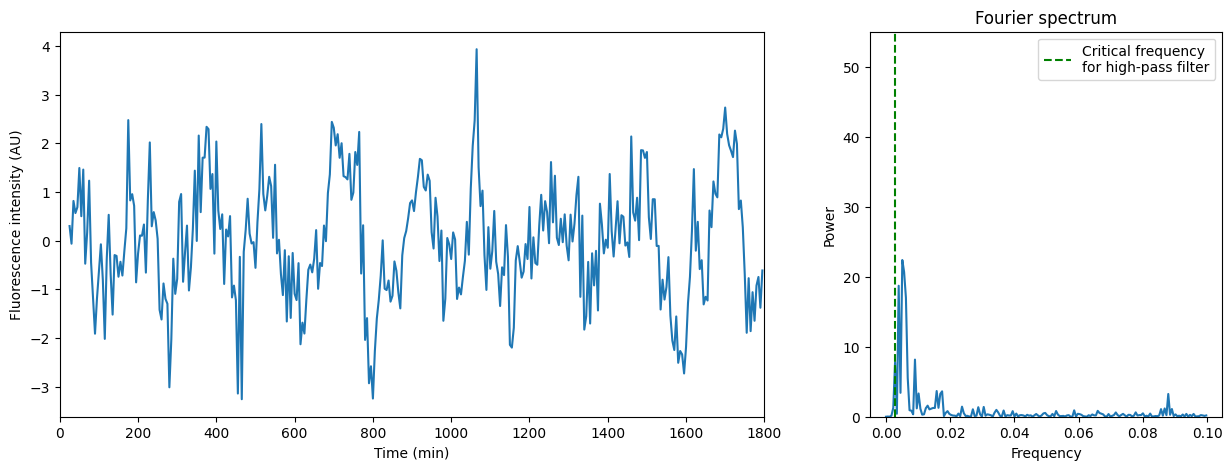
\includegraphics[width=\textwidth]{fft_butterworth}
   \caption{
     Signal processed with high-pass butterworth filter of frequency \SI[parse-numbers=false]{1/350}{\minute^{-1}}.
   }
   \label{fig:analysis-filter-butterworth}
  \end{subfigure}
  \begin{subfigure}[htpb]{0.8\textwidth}
   \centering
   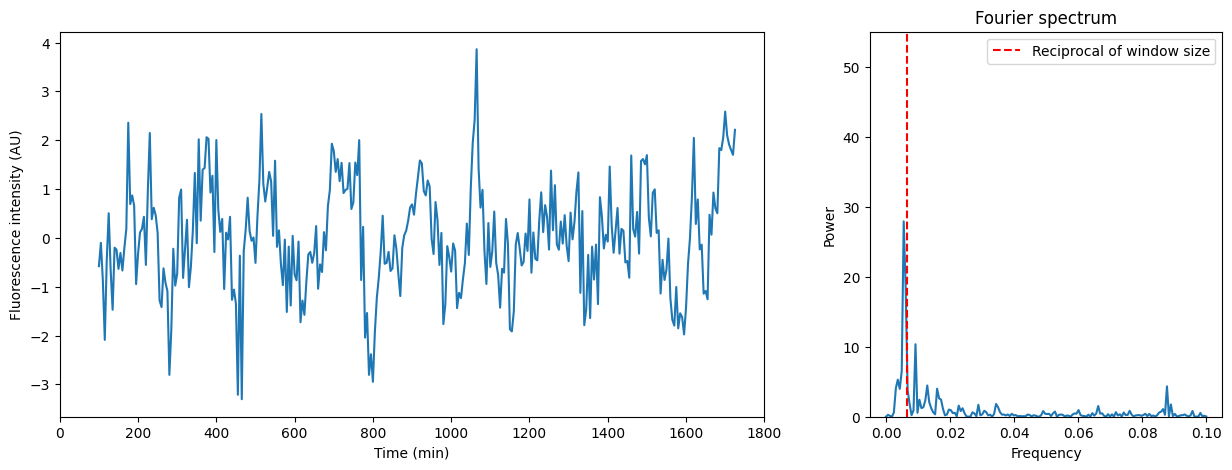
\includegraphics[width=\textwidth]{fft_slidingwindow}
   \caption{
     Signal processed by subtracting moving average with window size 30.
   }
   \label{fig:analysis-filter-slidingwindow}
  \end{subfigure}
  \begin{subfigure}[htpb]{0.8\textwidth}
   \centering
   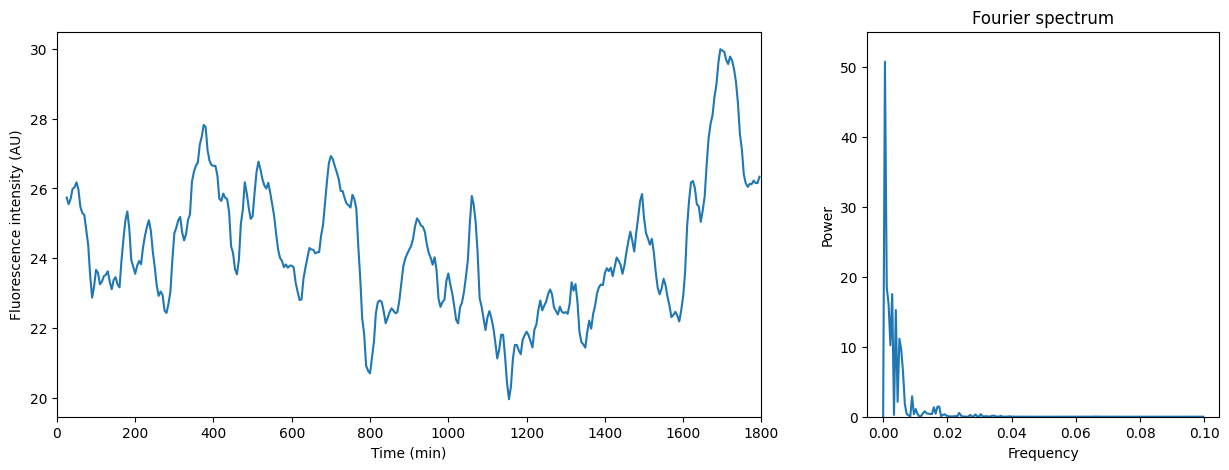
\includegraphics[width=\textwidth]{fft_savgol}
   \caption{
     Signal processed with Savitzky-Golay filter (window size 7, polynomial order 3).
   }
   \label{fig:analysis-filter-savgol}
  \end{subfigure}
  \caption[
    Different filtering methods
  ]{
    Different filtering methods result in different effects to both the signal (left panels) and the Fourier spectrum of the signal (right panels).
  }
  \label{fig:analysis-filter}
\end{figure}

For filtering time series, I have considered sliding-window methods and methods that modify the frequency profile of the time series.

Alternatively, I consider methods that modify the frequency profile of the time series.
Defining a high- or low-pass filter offers direct control over frequencies, but the user must use a judgement call to define a critical frequency.
In my case, I define the critical frequency for a high-pass Butterworth filter as \SI[parse-numbers=false]{1/350}{\minute^{-1}} as this corresponds to the upper limit of reasonable durations of yeast metabolic cycles and cell division cycles that I have observed in my single-cell microfluidics experiments (figure~\ref{fig:analysis-filter-butterworth}).
Defining a critical frequency in such a way will exclude the possibility of metabolic cycles that go on for longer; however, this is a trade-off I am willing to make so that I can extract the individual oscillations better.

Thus, for subsequent analysis, I use the high-pass Butterworth filter defined above to process raw fluorescence time series.
This is because using this method, I have more control over the frequency components, and the methods preserves noise frequencies that are useful for assessing the quality of the data set (to be discussed later in this section) and estimating the noise properties (to be discussed in section~\ref{subsec:analysis-characterisation-acf}).

However, sliding-window methods have caveats.
Subtracting a moving average relies on knowing a window size that approximates the expected oscillation period, gives no control over the signal frequencies, introduce artefacts in the frequency spectrum, and decreases the number of time points available (figure~\ref{fig:analysis-filter-slidingwindow}).
Such methods may distort the data in a way that affects conclusions.
Additionally, if the time series is processed with such methods, it is not possible to restore the raw data.


% However, there are challenges with classification of noisy biological time series with relatively few time points.
% In addition, such a classification task necessarily needs a cut-off somewhere, thus requiring judgement calls.
% You'd see this crop up in this section multiple times when I discuss my methods and I reveal different angles of approaching this.

Determining whether a time series is oscillatory, or rhythmicity detection, is technically difficult for several reasons.
From a signal processing perspective, any time-dependent signal can be decomposed into a combination of sinusoids of different frequencies.
Noise typically manifests as high-frequency components while trends manifests as low-frequency components --- the filtering methods in section~\ref{sec:analysis-cleaning} arise because of this fact.
It is thus more reasonable to detect the presence of a frequency within the range of interest.
However, this depends on knowing an expected range of frequencies.
When studying the circadian rhythm, this is often the case: studies expect rhythms of around \SI{24}{\hour} and \textcite{zielinskiStrengthsLimitationsPeriod2014} uses the range of \SIrange{16}{32}{\hour} for rhythmicity detection.
This method is less useful when the frequency of oscillations is unknown or known to be in a wide range of frequencies, as is the case for the yeast metabolic cycle.
Furthermore, there is no way to objectively specify a failure rate for a rhythmicity detection method as there is no independent method to estimate rhythmicity \parencite{zielinskiStrengthsLimitationsPeriod2014}, therefore such a classification method requires a subjective definition of whether each time series is oscillatory.
In other words, this is similar to the requirement of a training data set with human-defined labels, and thus a human-defined failure rate, for supervised machine learning.

%I then compared the classification results against manual classification of these time series into oscillating and non-oscillating.
The classifier was able to rank the time series by quality of oscillation (Fig.\ \ref{fig:ClassifierBestWorstTS}).
The peak of the normalised classical periodogram of each time series was used as a proxy for the quality of oscillation (Fig.\ \ref{fig:ClassifierBestWorstPS}).
By eye, birth events coincided with peaks of some higher-quality oscillations.
However, this was also true for some oscillations ranked as lower-quality.
% [COMMENTED -- don't think this sentence is really consequential, and the proposed plot doesn't add much] Additionally, higher-quality oscillations do not seem to be associated with imaging positions/flavin LED exposure times. % FIGURE: scatter plot, horizontal axis is rank, vertical axis is imaging position
% Wee bit of discussion (plus a plot to illustrate my point).  Deeper discussion about multiple main frequencies is in discussion, and has references to literature.
